\chapter{绪\hskip 0.4cm 论}
\label{ch1}

\section{研究背景及意义}
随着机器学习的不断发展和壮大,我们一方面惊叹于它的成就,比如Alpha GO击败了围棋世界冠军柯洁,或者面部识别技术帮助我们抓住了躲藏多年的逃犯,而大型工业企业也大力推动机器学习技术的应用。另一方面,我们也必须认识到,它的巨大潜力还有待实现,例如:构建基于大量病例的医疗救助诊断系统,运行基于大量商业行为数据的信用风险控制模型,帮助高价值企业融资,并基于整个产业链的数据提供个性化的产品分配和营销策略。我们真正见证了人工智能(AI)的巨大潜力,以及已经开始期待在许多应用中使用更复杂、更尖端的人工智能技术,包括无人驾驶、医疗、金融等今天,人工智能技术几乎在各方面都大显身手。传统的机器学习方法依赖于集中管理的训练数据集,建立在大量数据上,从数据中学习特征,从而完成复杂的任务,甚至是人类也难以完成的操作。

大多数训练数据是由不同组织的个人或部门产生的,一个AI项目可能涉及多个领域,需要融合各个公司、各个部门的数据。(比如研究居民线上消费问题,需要各个消费平台的数据,可能还需要银行数据等等),但在现实中想要将分散在各地、各个机构的数据进行整合几乎是不可能的。传统的机器学习是通过收集数据并将其发送到一个能看到并控制所有数据的中央服务器来完成的。因此,这个中心位置不仅要有强大的计算机集群来训练和创建机器学习模型,还要处理敏感数据并防止数据被用于其他目的。此外,敏感数据的处理方式必须不损害用户的隐私。然而,这用户完全信任服务器的假设已不再适用。在这种情况下,数据拥有者倾向于将数据掌握在自己手中,这就导致了孤立的数据孤岛,数据孤岛\cite{ref1}使所有利益相关者无法获得更多的数据。例如,每家医院的居民医疗记录的样本量完全不够,导致模型有偏差。在信贷领域,银行只能使用中央银行的信贷报告来建立风险控制模型。

然而,这些数据的采集可能涉及到用户的隐私,随着人们的隐私意识的普遍提高,相关的隐私法律法规的不断完善,中国出台的《网络安全与数据合规》白皮书中明确要求加强用户个人信息保护。2018年欧洲联盟出台《通用数据保护条例》中强调保护用户的个人隐私和数据安全用户可以删除或撤回其个人数据。近年来,也有越来越多的涉及数据泄漏和隐私侵权的事情,用户们也越来越关注自己的隐私信息是否在未经个人许可,或者出于商业和政治目的被他人或机构利用。随着个人意识和国家政策的关注,在大数据和人工智能领域数据采集和使用的过程中,保护用户隐私和数据的机密显得越来越重要。

人工智能的力量是基于大数据的,但我们被更多的小数据包围在孤岛中。大数据的基础就没有了,人工智能的基础也没有了。大数据的基础已经消失,人工智能的未来也岌岌可危。要解决大数据的困境,仅仅靠传统的方法已经出现瓶颈。两个公司简单的交换数据在很多法规包括《通用数据保护条例》是不允许的。用户是原始数据的拥有者,在用户没有批准的情况下,公司间不能交换数据。传统的机器学习和深度学习的方法本身已经成为解决大数据困境的绊脚石。简单地在两家公司之间交换数据,无论是《通用数据保护条例》还是GDPR\cite{ref2}都是不允许的:用户是原始数据的所有者,未经其同意,数据不能在公司之间交换。

那如何创建一个机器学习框架,使人工智能系统能够更有效和准确地集体使用数据,同时满足隐私、安全和监管要求,并解决数据孤岛的问题。如何才能做到这一点呢?

为了解决这个问题,google在2016年率先提出了联邦学习的概念\cite{ref3},它提供了一个具有隐私保护功能的分布式机器学习框架,并且能够以分布式方式与成千上万的参与者协作,迭代训练一个特定的机器学习模型。由于训练数据在联合过程中保持在参与者的本地,这种机制允许参与者之间共享训练数据,同时确保每个参与者的隐私。
如图所示,联合学习的基本工作流程如下:
(1) 初始化:所有用户在他们的设备上都有一个预先分配的神经网络模型,并且可以自愿加入联邦学习协议,指定相同的机器学习和模型训练目标。
(2) 本地训练:在一个给定的通信回合中,联邦参与者首先从中央服务器下载全局模型参数,然后使用他们的私人训练模式训练模型,创建本地模型更新(即模型参数),并将这些更新发送到中央服务器。
(3) 模型平均化:下一轮的全局模型是通过汇总所有通过训练不同的训练模式获得的模型更新并取其平均值来确定的。
(4) 迭代地执行上述步骤以达到优化当前全局模型的目的,整个迭代过程将在全局模型参数满足收敛条件时停止。

\begin{figure}[!hbt]
\centering
	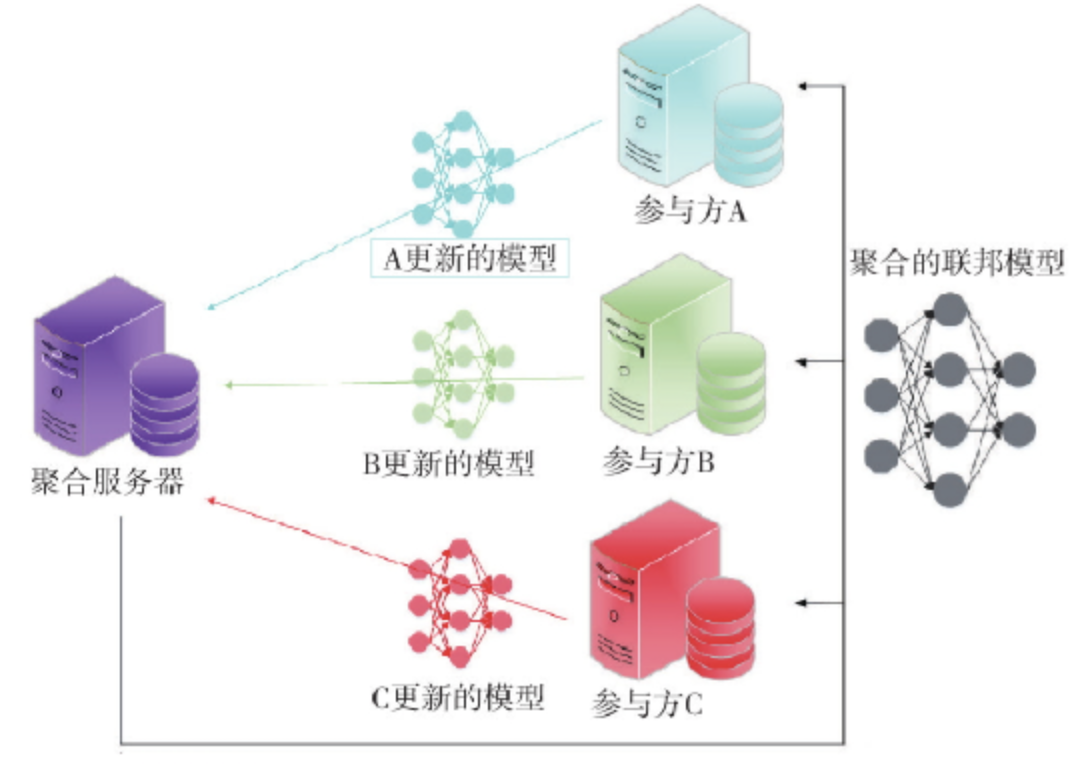
\includegraphics[scale=0.2]{fig2/C1/联邦学习概况}%联邦学习的系统架构
	\caption{联邦学习模型概况}
	\label{fig:联邦学习模型概况}	
\end{figure}

联合学习在隐私敏感的场景(包括金融、工业和许多其他与数据相关的场景)中显示出巨大的前景,这是因为它具有独特的优势,能够从多个参与者的本地数据中训练出一个统一的机器学习模型,同时保护数据隐私\cite{ref4}。联合学习解决了数据聚合的问题,并允许一些机器学习模型和算法在各机构和部门之间进行设计和训练。在一些移动设备上的机器学习模型应用中,联邦学习显示出良好的性能和稳健性。此外,对于一些没有足够的私人数据来开发准确的本地模型的用户(客户)来说,机器学习模型和算法的性能可以通过联合学习得到显著改善。

\section {问题和挑战}


\subsection{数据异构}
由于联邦学习的重点是通过以分布式方式从所有参与的客户端设备中学习本地数据来获得高质量的全局模型,所以它无法捕捉每个设备的个人信息,导致推理或分类性能下降。此外,传统的联邦学习要求所有参与的设备同意使用一个共同的模型来共同训练,这在复杂的现实世界物联网应用中是不现实的。研究人员对学习在实际应用中面临的问题总结如下\cite{ref5}。

(1)设备的异质性:由于客户端设备的硬件条件(CPU、内存)、网络连接(3G、4G、5G、WiFi)和电源(电池)的变化,联邦学习网络上每个设备的存储、计算和通信能力都可能不同。由于网络和设备的限制,在任何时候都只有某些设备可以活动。此外,设备可能会受到意外事件的影响,如断电或断网,这可能会导致暂时的断网。这种异质性的系统结构影响了联邦模型的整体学习战略。

(2)统计的异质性:在整个网络中,设备通常以不同的方式产生和收集数据,而且不同设备的数据量、特征等会有很大的不同,所以联邦学习网络中的数据不是独立和相同的分布(非IID)。目前,目前的机器学习算法主要是基于对IID数据的假想假设。因此,非IID数据的异质属性给建模、分析和评估带来了重大挑战。FederatedAverageing(FedAvg)方法来解决非均匀同分布数据的问题,但是当数据分布偏态很严重的时候FedAvg的性能退化严重,一方面其性能比中心化的方法差好多,另一方面它只能学习到IoT设备粗粒度的特征而无法学习到细粒度的特征。

(3)模型的异质性:每个客户根据其应用场景要求定制不同模型。

\subsection{高昂的通信代价}
在联邦学习过程中,根据存储在几十甚至几百万个远程客户端设备上的数据来学习一个全局模型。在训练期间,客户设备必须定期与中央服务器进行通信原始数据被储存在本地的远程客户端设备上,这些设备必须不断地与中央服务器互动,以完成全局模型的构建。通常情况下,整个联盟学习网络可能涉及大量的设备,而网络通信可能比本地计算慢几个数量级,因此高通信成本成为联邦学习的关键瓶颈。

\subsection{安全性和隐私威胁}

(1) 由于联合学习系统的云端服务器无法访问参与者的本地数据和他们的训练过程,恶意参与者可以发送无效的模型更新来达到并破坏全局模型。例如,内部攻击者可以通过在修改后的训练数据上引起有毒的模型更新来有效地损害全局模型的准确性。内部攻击可以由联邦学习服务器发起,也可以由联邦学习参与方发起。外部攻击(包括偷听者)通过参与方与服务器之间的通信通道发起。外部攻击的发起者大部分为恶意的参与方,例如敌对的客户、敌对的分析者、破坏学习模型的敌对设备或者其组合。在联邦学习中,恶意设备可以通过白盒或者黑盒的方式访问最终模型,因此在防范来自系统外部的攻击时,需要考虑模型迭代过程中的参数是否存在泄露原始数据的风险,这对严格的隐私保护提出了新的挑战。

(2) 由于局部模型更新和全局模型参数的结合提供了关于训练数据的隐藏知识,用户的个人信息有可能泄露给不受信任的服务器或其他恶意用户。例如,即使是由其他用户的训练数据生成的样本原型也会被恶意用户隐蔽地窃取。在训练过程中,攻击方可以试图学习、 影响或者破坏联邦学习模型。在联邦训练的过程中,攻击方可以通过数据中毒攻击的方式改变训练数据集合收集的完整性,或者通过模型中毒攻击改变学习过程的完 整性。攻击方可以攻击一个参与方的参数更新过程,也可以攻击所有参与方的参数更新过程。
若联邦学习的参与方想利用各方的数据集合训练一个模型,但是又不想让自己的数据集泄露给服务器,就需要约定联邦建模的模型算法(例如神经网络)和参数更新的机制(例如随机梯度下降(stochastic gradient descent,SGD))。那么在训练前,攻击方就可以获取联邦学习参数更新 的机制,从而指定对应的推断攻击策略。

(3) 在不信任的云服务器和恶意参与者的勾结下,任何个人的确切私人信息都会被泄露。


\section{国内外研究现状}
尽管联邦学习提供了隐私保护的机制,还是有各种类型的攻击方式可以攻击联邦学习系统,从而破坏联邦学习系统安全和参与方的隐私。本节将讨论关于联邦学习的攻击问题。从参与方的类型来看,可 以将联邦学习的威胁模型细分为半诚实模型 (semi-honest model)和恶意模型。对于联邦学习系统的攻击,本文按照不同的维度进行不同层次的分类。从攻击方向角度来看,可以将联邦学习的攻击分为从内部发起和从外部发起两个方面。从攻击者的角色角度来看,可以将攻击分为参与方发起的攻击、中心服务器发起的攻击和第三方发起的攻击。从发动攻击的方式角度来看,可以将攻击分为 中毒攻击和拜占庭攻击。从攻击发起的阶段角度,可以将攻击分为模型训练过程的攻击和模型推断过程的攻击。在密码学领域,基于模型安全的假设通常可以被分为半诚实但好奇(onest but curious)的攻击方假设以及恶意攻击方假设。

\subsection{隐私威胁的研究现状}
各类攻击模型阻碍了深度学习技术的发展,也会极大地威胁到人们的隐私敏感信息。无论是模型并行化还是数据并行化,分布式学习系统在用户数据隐私性方面相对于集中式学习存在一定的优势 。但\cite{ref6}发现, 在分布式联邦学习系统中, 参与者需要多次的联合迭代过程才能完成全局模型的收敛, 参与者的参数也需要多次的训练、上传和共享, 这些参数中包含的参与者训练集的相关信息, 用户的信息可以通过计算用户上传的多个参数得到。

模型反演攻击:\cite{ref7}利用这样的参数信息,以一种很简单的方式攻击用户数据:一旦用户的网络模型经过训练并达到收敛,攻击者就可以通过调整网络模型权重的梯度, 获得网络模型中所有表示类的逆向工程试例。在模型反演攻击中, 攻击者无需接触目标信息的标签类,攻击模型仍然能够恢复原始样本试例。这一攻击模型表明,任何经过精确训练的深度学习网络,无论是以何种方式进行训练收敛, 都可以泄露深度网络中区分不同标签类的信息。但是参数中包含的信息有限,模型反演攻击方式很难攻击卷积神经网络等复杂深度网络模型,在模型进行了 一定的隐私保护后,攻击也基本失效。

GAN攻击:目前研究人员也利用诸多安全模型对深度学习网络的训练数据集进行保护,但Hitaj等人\cite{ref8}发现,一个联邦学习框架非常容易受到系统内参与者发起的主动攻击。他们首先提出了一个由系统内的恶意用户发起的基于GAN的重建攻击。在训练阶段,攻击者可以冒充无害的用户,训练GAN来模拟由其他用户的训练数据产生的原型样本。通过不断添加假的训练样本,攻击可以逐渐影响整个学习过程,使受害者暴露出更多关于攻击者的目标类的敏感信息。除了客户端发起的GAN攻击,服务器也能通过GAN攻击。恶意服务器最初假装是一个为用户提供联邦学习服务的正常服务器,但其主要目标是重建被攻击用户的训练样本。

模型反演攻击:在联邦学习框架中,攻击者可能试图修改、删除或插入恶意信息到训练数据中,以破坏原始数据分布,改变学习算法的逻辑.两种常见的中毒攻击的例子包括标签翻转攻击\cite{ref9}和后门攻击\cite{ref10}。标签反转攻击是指恶意用户反转样本标签,并在训练数据中加入预定义的攻击点,导致训练后的模型偏离预测的界限。与标签反转攻击不同,后门要求攻击者用精心设计的训练数据,利用特定的隐藏模式来训练目标的深度神经网络(DNN)模型。这些模型被称为 "反馈回路",可以干扰学习模型,并在预测阶段产生与真实情况截然不同的结果。

如上文所述,联邦学习机制要求所有参与者通过在本地数据集上训练全局模型来更新梯度。在这种情况下,如果联邦学习系统有一个不被信任的服务器,其知识不能被信任,那么用户的私人信息就不能得到保证。这个不受信任的服务器可以获得关于每个参与者的本地训练模型的大量额外信息(例如,模型结构、用户身份和梯度),并且能够充分损害用户的隐私信息。具体实现如下:攻击者首先在平均化后获得模型的全局参数,并在本地存储这些快照。然后,通过计算以下快照与进一步获取用户的隐私信息。

\subsection{隐私保护的研究现状}
在联邦学习中,存在着无数与隐私有关的挑战学习中的隐私问题。除了保证隐私之外,重要的是要保证确保通信成本的低廉和高效。有许多关于联邦学习的隐私定义\cite{ref11}\cite{ref12}\cite{ref13}。我们可以把它们分为两类:局部隐私和全局隐私。在本地隐私中,每个客户端发送一个不同的隐私值,该值是安全的加密的到服务器。在全局模型中,服务器在最终输出中添加不同的隐私噪音。安全多方计算、同态加密和差分隐私是最常见的保证联邦学习中的安全和隐私的技术。

安全多方计算模型涉及多方,并在一个定义明确的模拟框架中提供安全证明,以保证完全的零知识,即每一方除了其输入和输出外一无所知。零知识是非常理想的,但这种理想的属性通常需要复杂的计算协议,而且可能无法有效实现。在某些情况下,如果提供安全保证,部分知识的披露可能被认为是可以接受的。有可能在较低的安全要求下建立一个具有SMC的安全模型,以换取效率\cite{ref14}。在\cite{ref15}中,MPC协议被用于模型训练和验证,而用户不会泄露敏感数据。最先进的SMC框架之一是Sharemind\cite{ref16}。\cite{ref17}的作者提出了一个具有诚实多数的3PC模型\cite{ref18},并考虑了半诚实和恶意假设的安全性。这些作品要求参与者的数据在非共存的服务器之间秘密共享。

同态加密是一种加密形式,它允许人们对密文进行特定形式的代数运算得到仍然是加密的结果,将其解密所得到的结果与对明文进行同样的运算结果一样同态加密\cite{ref19},明文通过同态加密方法得到密文后,可实现密文间的计算(密文计算后解密的结果等价于明文计算的结果)。如果对密文进行加法(或乘法)运算后解密,与明文进行加法(或乘法)运算,结果相等,则称这种加密算法为加法(乘法)同态。如果同时满足加法和乘法同态,则称为全同态加密。在联邦学习中,因为只需要对中间结果或模型进行聚合,一般使用的同态加密算法为PHE(多见为加法同态加密算法),通过加密机制下的参数交换来保护用户数据隐私\cite{ref20},例如在FATE中使用的Paillier即为加法同态加密算法。

差分隐私方法涉及向数据添加噪音,或使用概括方法来掩盖某些敏感属性,直到第三方无法区分个人,从而使数据无法被还原以保护用户的隐私。利用差分隐私,可以在本地模型训练及全局模型整个过程中对相关参数进行扰动,从而令敌手无法获取真是模型参数,但是与密码学技术相比,差分隐私无法保证参数传递过程中的机密性,从而增加了模型遭受隐私攻击的可能性.例如刘俊旭等人\cite{ref21}针对联邦学习下差分隐私中存在的攻击方法进行了详细的调研。在\cite{ref22}中,作者为联合学习引入了一种差异化的隐私方法,以便通过在训练期间隐藏客户端的贡献来增加对客户端数据的保护。在深度学习中,差分隐私可以作为一种局部隐私保护方案来保护用户梯度的隐私,Abadi等人\cite{ref23}提出了一种隐私保护的深度学习方法,主要通过使用噪声来扰乱少量步骤后的局部梯度,将差分隐私机制与SGD算法相结合。令人担忧的是,隐私保护预算的成本和联合学习的有效性之间的权衡是困难的,因为较高的隐私保护预算可能对一些大规模的攻击(如基于GAN的攻击)不是很有用\cite{ref24},而较低的隐私保护预算可能阻碍模型的局部收敛。


总的来说,安全多方计算基于复杂的计算协议,同态加密的运算成本非常高,而差分隐私破坏了数据的可用性,很难在模型性能和隐私成本上达到平衡,当前的研究方向主要集中在对数据集和神经网络中的参数的加密和隐私保护机制上,较少关注到模型整体框架等过程。目前的联邦学习中的隐私保护方法还有许多不足,不能在隐私性和模型可用性上都达到一个相对满意的效果,此外, 大部分方法是基于统一的、固定的参数设置,会导致模型迭代过程中累积大量隐私损失,使模型性能大幅下降。因此,在联邦学习场景下,保护用户隐私的同时保持模型准确性仍需大量的研究。


\section{本文工作与主要贡献}
针对联邦学习中隐私性和模型精度的双重指标,本文提出了本地自适应差分隐私算法和安全混洗框架,主要的工作和贡献包含以下三个方面:
\begin{enumerate}
\item [(1)] 在联邦学习差分隐私的场景下,本文提出了一种新型的、基于本地差分隐私的权重分配自适应干扰算法。在客户端本地训练的神经网络模型中,通过改进层间依赖传播算法,计算每个属性类对于模型输出的贡献比,然后,我们开发了一个自适应噪声添加的方案,根据贡献率注入不同隐私预算的噪声。与传统的注入噪声的方法相比,我们在相同的隐私保护程度下最大限度地提高了模型的准确性,减少噪声对模型输出结果的影响,提高模型精度。
\item [(2)] 考虑到联邦学习中参数聚合器的攻击,本文提出了一种新的安全聚合机制,在本地客户端和中心服务器之间新增混洗器,在用户将参数上传到云服务器之前,先对参数进行混洗,模型参数的更新被匿名的发送到混洗器,通过对模型参数的拆分和混洗实现客户端匿名,并在联邦学习中改进基于稀疏向量技术的差分隐私进行保护,并且证明了安全混洗模型的可行性。
\item [(3)] 本文通过实验,展示了自适应本地差分隐私方案和安全混洗框架的结合,使得联邦学习的模型的精度和隐私预算达到平衡。
\end{enumerate}

\section{本文组织结构}

本文一共六章,主要内容的组织安排如下:

第一章对本文研究内容:联邦学习的研究背景和实际意义进行了阐述,介绍了目前联邦学习中的隐私保护的研究现状和发展方向。

第二章详细介绍本文研究内容所涉及的一些理论基础与背景知识,包含了联邦学习的相关概念,差分隐私的基础知识和神经网络的基本结构。

第三章描述了本文所提出的本地自适应差分隐私算法的设计和实现,根据神经网络层间依赖传播算法,分析属性值的贡献度,并分析了在差分隐私机制下的联邦学习算法的收敛性和隐私性。
  
第四章在上一章的基础之上,提出了一种联邦学习安全混洗模型,在联邦学习中改进基于稀疏向量技术的差分隐私进行保护,再将混洗模型和自适应本地差分隐私保护方法结合在分布式系统中,提高系统学习效果。并且证明了安全混洗模型的可行性。
    
第五章为实验部分,基于本文提出的隐私保护框架,我们在三个基准数据集的进行了实验和讨论,并与之前的差分隐私联邦学习框架进行对比实验。

第六章是对本文的一个内容总结和展望,首先对本文的研究内容进行了概括,并对现有的不足进行总结,对未来的研究和改进方向进行了展望。

\section{本章小结}
这一章节为绪论,主要介绍的是本文章的研究背景以及意义,对当下联邦学习中的应用以及存在的问题与挑战行了介绍和总结、讨论了联邦学习中隐私威胁和隐私保护的国内外研究现状,并对文章的主要工作和文章的章节进行了介绍。

